%% -*- Lecture -*-

\synctex=1
\documentclass[11pt]{beamer}

\usepackage[oldspacing]{lectureb}
\usetheme{lectureb}
\topic{Protection}

\usepackage{tikz}
\usetikzlibrary{shapes,shadows.blur,positioning,fit,backgrounds}

\begin{document}

\begin{slide}{View access control as a matrix}
\centerline{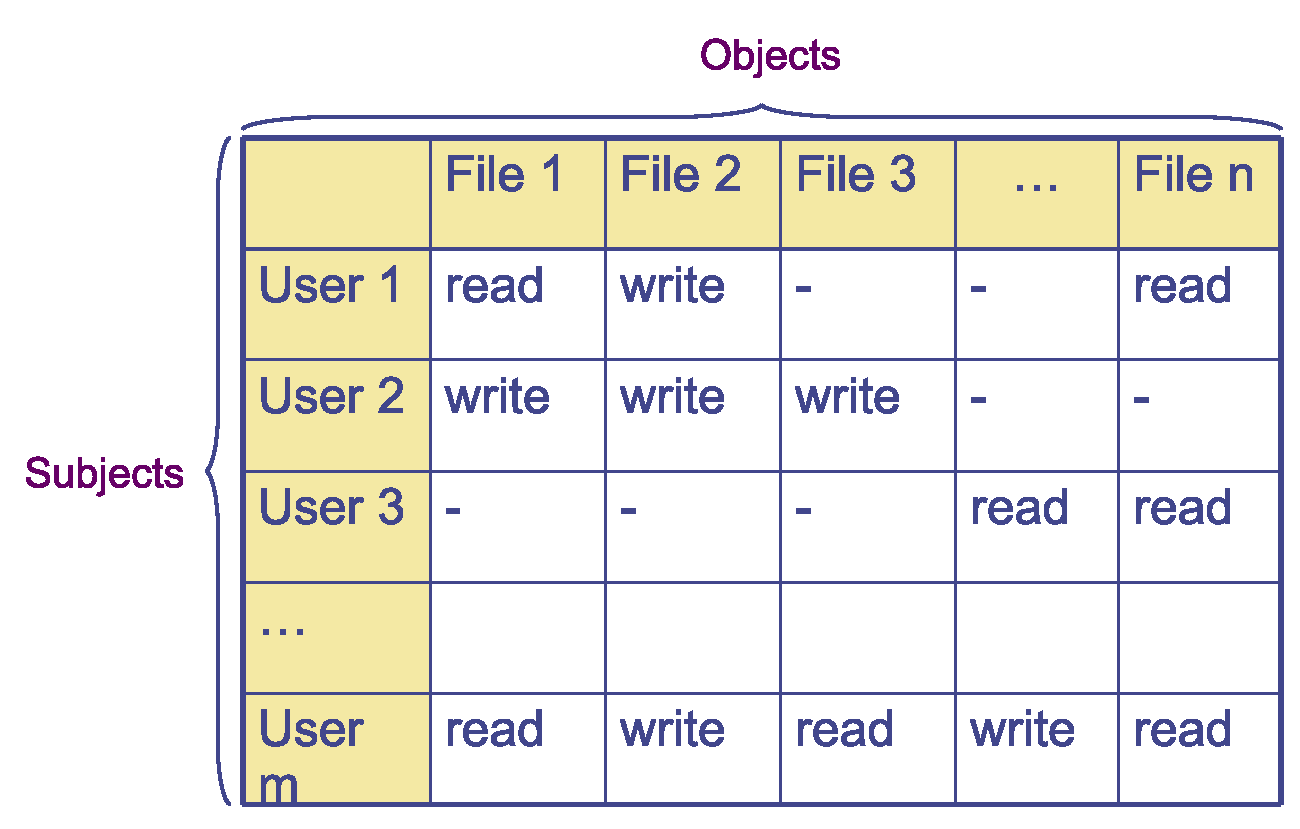
\includegraphics[width=4in]{figs/matrix}}
\itms{
  \item Subjects (processes/users) access objects (e.g., files)
  \item Each cell of matrix has allowed permissions
}
\end{slide}

\begin{slide}{Specifying policy}
\itms{
  \item Manually filling out matrix would be tedious
  \item Use tools such as groups or \emph{role-based access control}:
}
\centerline{\includegraphics[width=4in]{rbac}}
\end{slide}

\begin{slide}{Two ways to slice the matrix}
\itms{
  \item Along columns:
  \ittms{
    \item Kernel stores list of who can access object along with object
    \item Most systems you've used probably do this
    \item Examples:  Unix file permissions, Access Control Lists (ACLs)
  }
  \item Along rows:
  \ittms{
    \item Capability systems do this
    \item More on these later\ldots
  }
}
\end{slide}

\section{Unix/Linux protection}

\begin{slide}{Example:  Unix protection}
\itms{
  \item Each process has a User ID \& one or more group IDs
  \item System stores with each file:
  \ittms{
    \item User who owns the file and group file is in
    \item Permissions for user, any one in file group, and other 
  }
  \item Shown by output of \texttt{ls -l} command:
  \ittms{
    \item[] $\texttt{-}%\overbrace{\texttt{-}}^\mathrm{type}
      \overbrace{\texttt{rw-}}^\mathrm{user}
      \overbrace{\texttt{rw-}}^\mathrm{group}
      \overbrace{\texttt{r--}}^\mathrm{other}
      \overbrace{\texttt{dm}}^\mathrm{owner}
      \overbrace{\texttt{cs140}}^\mathrm{group}$
      \texttt{ ... index.html}
    \item Each group of three letters specifies a subset of \\
      \texttt{\Red{r}ead}, \texttt{\Red{w}rite}, and
      \texttt{e\Red{x}ecute} permissions
    \item User permissions apply to processes with same user ID
    \item Else, group permissions apply to processes in same group
    \item Else, other permissions apply
  }
}
\end{slide}

\begin{slide}{Unix continued}
\itms{
  \item Directories have permission bits, too
  \ittms{
    \item Need write permission on a directory to create or delete a file
  }
  \item Special user \texttt{root} (UID 0) has all privileges
  \ittms{
    \item E.g., Read/write any file, change owners of files
    \item Required for administration (backup, creating new users,
  etc.)
  }
  \item Example:
  \ittms{
    \item \texttt{drwxr-xr-x 56 root wheel 4096 Apr  4 10:08 /etc}
    \item Directory writable only by root, readable by everyone
    \item Means non-root users cannot directly delete files in \texttt{/etc}
    \item E\Red{x}ecute permission means ability to use pathnames in
      the directory, separate from \Red{r}ead permission which allows
      listing
  }
}
\end{slide}

\begin{slide}{Non-file permissions in Unix}
\itms{
  \item Many devices show up in file system
  \ittms{
    \item E.g., \texttt{/dev/tty1} permissions just like for files
  }
  \item Other access controls not represented in file system
  \item E.g., must usually be root to do the following:
  \ittms{
    \item Bind any TCP or UDP port number less than 1,024
    \item Change the current process's user or group ID
    \item Mount or unmount file systems
    \item Create device nodes (such as \texttt{/dev/tty1}) in the file system
    \item Change the owner of a file
    \item Set the time-of-day clock; halt or reboot machine
  }
}
\end{slide}

\begin{slide}{Example: Login runs as root}
\itms{
  \item Unix users typically stored in files in \texttt{/etc}
  \ittms{
    \item Files \texttt{passwd}, \texttt{group}, and often
      \texttt{shadow} or \texttt{master.passwd}
  }
  \item For each user, files contain:
  \ittms{
    \item Textual username (e.g., ``\texttt{dm}'', or ``\texttt{root}'')
    \item Numeric user ID, and group ID(s)
    \item One-way hash of user's password:
      $\{\mathrm{salt},H(\mathrm{salt},\mathrm{passwd})\}$
    \item Other information, such as user's full name, login shell, etc.
  }
  \item \texttt{/usr/bin/login} runs as root
  \ittms{
    \item Reads username \& password from terminal
    \item Looks up username in \texttt{/etc/passwd}, etc.
    \item Computes $H(\mathrm{salt}, \mathrm{typed\ password})$ \&
      checks that it matches
    \item If matches, sets group ID \& user ID corresponding to username
    \item Execute user's shell with \texttt{execve} system call
  }
}
\end{slide}


\begin{slide}{Setuid}
\itms{
  \item Some legitimate actions require more privs than UID
  \ittms{
    \item E.g., how should users change their passwords?
    \item Stored in root-owned \texttt{/etc/passwd} \&
  \texttt{/etc/shadow} files
  }
  \item Solution:  Setuid/setgid programs
  \ittms{
    \item Run with privileges of file's owner or group
    \item Each process has \emph{real} and \emph{effective} UID/GID
    \item \emph{real} is user who launched setuid program
    \item \emph{effective} is owner/group of file, used in access checks
    \item Actual rules and interfaces somewhat complicated
      \href{http://www.cs.berkeley.edu/~daw/papers/setuid-usenix02.pdf}{[Chen]}
  }
  \item Shown as ``s'' in file listings
  \ittms{
    \item \texttt{-rw\Red{s}--x--x 1 root root 38464 Jan 26 14:26 /bin/passwd}
    \item Obviously need to own file to set the setuid bit
    \item Need to own file and be in group to set setgid bit
  }
}
\end{slide}

\begin{slide}{Setuid (continued)}
\itms{
  \item Examples
  \ittms{
    \item \texttt{passwd} -- changes user's password
    \item \texttt{su} -- acquire new user ID (given correct password)
    \item \texttt{sudo} -- run one command as root
    \item \texttt{ping} -- uses raw IP sockets to send/receive ICMP packets
%    \item \texttt{netstat} -- lists network
%      connections (by reading kernel memory on some OSes)
  }
  \item Have to be very careful when writing setuid code
  \ittms{
    \item Attackers can run setuid programs any time (no need to wait
          for root to run a vulnerable job)
    \item Attacker controls many aspects of program's environment
  }
  \item Example attacks when running a setuid program
  \ittms{
    \item Change PATH or IFS if setuid prog calls system(3)
    \item Set maximum file size to zero (if app rebuilds DB)
    \item Close fd 2 before running program---may accidentally send
      error message into protected file
  }
}
\end{slide}

\begin{slide}{Other permissions}
\itms{
  \item When can proc.\ $A$ send a signal to proc.\ $B$
    w.\ \emph{kill}?
  \ittms{
    \item Allow if sender and receiver have same effective UID
    \item But need ability to kill processes you launch
      even if suid
    \item So allow if real UIDs match, as well
    \item Can also send SIGCONT w/o UID match if in same session
  }
  \item Debugger system call \emph{ptrace}
  \ittms{
    \item Lets one process modify another's memory
    \item Setuid gives a program more privilege than invoking user
    \item So don't let process ptrace more privileged process
    \item E.g., Require sender to match real \& effective UID of target
    \item Also disable/ignore setuid if ptraced target calls \emph{exec}
    \item Exception:  root can \emph{ptrace} anyone
  }
}
\end{slide}

\section{Unix/Linux security holes}

\begin{slide}{A security hole}
\itms{
\item \Red{Even without root or setuid, attackers can trick root owned
  processes into doing things\ldots}
\item Example: Want to clear unused files in \texttt{/tmp}
\item Every night, automatically run this command as root:
\ittms{
\item[]
\texttt{find /tmp -atime +3 -exec rm -f -{}-
\char`\{\char`\}\ \char`\\;}}
\item \textsf{find} identifies files not accessed in 3~days
\ittms{
  \item executes \textsf{rm}, replacing $\{\}$ with file name
}
\item \textsf{rm -f -{}-} \textit{path} deletes file \textit{path}
\ittms{
  \item Note ``-{}-'' prevents \textit{path} from being parsed as option
}
\item What's wrong here?
}
\end{slide}

\begin{slide}{An attack}
\centerline{\small\sf
\begin{tabular}{l@{\quad}l}
\textbf{find/rm} & \textbf{Attacker} \\
\omit~~\hrulefill\quad& \hrulefill \\[.1pt]
& mkdir (``\texttt{/tmp/\Green{badetc}}'') \\
& creat (``\texttt{/tmp/\Green{badetc}/passwd}'') \\
readdir (``\texttt{/tmp}'') $\to$ ``\texttt{\Green{badetc}}'' & \\
lstat (``\texttt{/tmp/\Green{badetc}}'') $\to$ \textsc{directory} & \\
readdir (``\texttt{/tmp/\Green{badetc}}'') $\to$ ``\texttt{passwd}'' & \\
& \onslide<2->{rename (``\texttt{/tmp/\Green{badetc}}'' $\to$
    ``\texttt{/tmp/x}'')} \\
& \onslide<2->{symlink (``\texttt{/\Red{etc}}'',
    ``\texttt{/tmp/\Red{badetc}}'')} \\
unlink
(``\texttt{/tmp/\only<1>{\Green{badetc}}%
    \only<2->{\Red{badetc}}/passwd}'') & \\
\end{tabular}}
%\itms{\item Solution: Syscalls use immutable names}

\vspace*{.2in}
\pause
\itms{
  \item Time-of-check-to-time-of-use
    \cref{sched/readings/tocttou.pdf}{[TOCTTOU]}
      bug
  \ittms{
    \item \textsf{find} checks that \texttt{/tmp/badetc} is not symlink
    \item But meaning of file name changes before it is used
  }
}
\end{slide}

\defverbatim[colored]\VerbEnvOne{
\begin{ccode}
        if (access (logfile, W_OK) < 0)
          return ERROR;
\end{ccode}}
\defverbatim[colored]\VerbEnvTwo{
\begin{ccode}
        fd = open (logfile, O_CREAT|O_WRONLY|O_TRUNC, 0666);
        /* ... */
\end{ccode}}

\begin{slide}{xterm command}
\itms{
  \item Provides a terminal window in X-windows
  \item Used to run with setuid root privileges
  \ittms{
    \item Requires kernel pseudo-terminal (pty) device
    \item Required root privs to change ownership of pty to user
    \item Also writes protected utmp/wtmp files to record users
  }
  \item Had feature to log terminal session to file
}
\onslide<2->{\VerbEnvOne}
\VerbEnvTwo
\itms{
\only<1>{\item What's wrong here?}
\onslide<2->
  \item \texttt{xterm} is root, but shouldn't log to file user can't
    write
  \item \texttt{access} call avoids dangerous security hole
  \ittms{
    \item Does permission check with \emph{real}, not \emph{effective} UID
      \onslide<3->
    \item \Red{\textbf{Wrong:  Another TOCTTOU bug}}
  }
}
\end{slide}

\begin{slide}{An attack}
\vspace*{-.2in}
{\small\sf
\begin{tabular}{l@{\qquad}l}
\textbf{xterm} & \textbf{Attacker} \\
\omit~~\hrulefill\quad& \hrulefill \\[.1pt]
& creat (``\texttt{/tmp/\Green{X}}'') \\
access (``\texttt{/tmp/\Green{X}}'') $\to$ OK \\
& unlink (``\texttt{/tmp/\Green{X}}'') \\
& symlink (``\texttt{/tmp/\Red{X}}'' $\to$
	``\texttt{/etc/\Red{passwd}}'') \\
open (``\texttt{/tmp/\Red{X}}'') \\
\end{tabular}}

\smallskip

\itms{
  \item Attacker changes \texttt{/tmp/X} between check and use
  \ittms{
    \item \textsf{xterm} unwittingly overwrites \texttt{/etc/passwd}
    \item Another TOCTTOU bug
  }
\item OpenBSD man page:  ``CAVEATS:  access() is a potential security hole
and should never be used.''}
\end{slide}

\begin{slide}{{}SSH configuration files}
\itms{
  \item SSH 1.2.12 client ran as root for several reasons:
  \ittms{
    \item Needed to bind TCP port under 1,024 (privileged operation)
    \item Needed to read client private key (for host authentication)
  }
  \item Also needed to read \& write files owned by user
  \ittms{
    \item Read configuration file \texttt{\char`\~/.ssh/config}
    \item Record server keys in \texttt{\char`\~/.ssh/known\_hosts}
  }
  \item Software structured to avoid TOCTTOU bugs:
  \ittms{
    \item First bind socket \& read root-owned secret key file
    \item Second drop \emph{all} privileges---set real,
      \& effective UIDs to user
    \item Only then access user files
    \item Idea: avoid using any user-controlled arguments/files until
          you have no more privileges than the user
    \item What might still have gone wrong?
  }
}
\end{slide}

\begin{slide}{Trick question:  ptrace bug}
\itms{
  \item Actually do have more privileges than user!
  \ittms{
    \item Bound privileged port and read host private key
  }
  \item Dropping privs allows user to ``debug'' SSH
  \ittms{
    \item Depends on OS, but at the time several had \emph{ptrace}
      implementations that made SSH vulerable
  }
  \item Once in debugger 
  \ittms{
    \item Could use privileged port to connect anywhere
    \item Could read secret host key from memory
    \item Could overwrite local user name to get privs of other user
  }
  \item The fix: restructure into 3 processes!
  \ittms{
    \item Perhaps overkill, but really wanted to avoid problems
  }
  \item Today some linux distros restrict ptrace with
    \href{https://www.kernel.org/doc/Documentation/security/Yama.txt}{Yama}
}
\end{slide}




\begin{slide}{A Linux security hole}
\itms{
  \item Some programs acquire then release privileges
  \ittms{
    \item E.g., \texttt{su user} is setuid root, becomes \texttt{user}
      if password correct
  }
  \item Consider the following:
  \ittms{
    \item A and B unprivileged processes owned by attacker
    \item A ptraces B (works even with Yama, as B could be child of A)
    \item A executes ``\texttt{su user}'' to its own identity
    \item With effective UID (EUID) 0, \texttt{su} asks for password \& waits
    \item While A's EUID is 0, B execs \texttt{su root}\\
      (B's exec honors setuid---not disabled---since A's EUID is 0)
    \item A types password, gets shell, and is attached to \texttt{su root}
    \item Can manipulate \texttt{su root}'s memory to get root shell
  }
}
\end{slide}

\begin{frame}
%\frametitle{\raise-.5in\hbox{\includegraphics[height=1in]{editorial}}}
\centerline{\begin{tikzpicture}[font=\LARGE\bfseries,text=beamer@blendedblue]
\node[starburst, double=white, fill=white, draw=yellow, ultra thick, blur shadow]
    {Editorial};
\end{tikzpicture}}
\itms{
  \item Previous examples show two limitations of Unix
  \item Many OS security policies \emph{subjective} not \emph{objective}
  \ittms{
    \item When can you signal/debug process? Re-bind network port?
    \item Rules for non-file operations somewhat incoherent
    \item Even some file rules weird (Creating hard links to files)
  }
  \item Correct code is much harder to write than incorrect
  \ittms{
    \item Delete file without traversing symbolic link
    \item Read SSH configuration file (requires 3 processes??)
    \item Write mailbox owned by user in dir owned by root/mail
  }
  \item Don't \emph{just} blame the application writers
  \ittms{
    \item Must also blame the interfaces they program to
  }
}
\end{frame}

\section{Capability-based protection}

\begin{slide}{Another security problem
    \cref{sched/readings/confused.pdf}{[Hardy]}}
\itms{
  \item Setting:  A multi-user time sharing system
  \ittms{
    \item This time it's not Unix
  }
  \item Wanted fortran compiler to keep statistics
  \ittms{
    \item Modified compiler \texttt{/sysx/fort} to record stats in
    \texttt{/sysx/stat}
    \item Gave compiler ``home files license''---allows writing to
  anything in \texttt{/sysx} (kind of like Unix setuid)
  }
  \item What's wrong here?
}
\end{slide}

\begin{slide}{A confused deputy}
\itms{
  \item Attacker could overwrite any files in \texttt{/sysx}
  \ittms{
    \item System billing records kept in \texttt{/sysx/bill} got wiped
    \item Probably command like \texttt{fort -o /sysx/bill file.f}
  }
  \item Is this a bug in the compiler \texttt{fort}?
  \ittms{
    \item Original implementors did not anticipate extra rights
    \item Can't blame them for unchecked output file
  }
  \item Compiler is a ``confused deputy''
  \ittms{
    \item Inherits privileges from invoking user (e.g., read \texttt{file.f})
    \item Also inherits privileges from home files license
    \item Which master is it serving on any given system call?
    \item OS doesn't know if it just sees \texttt{open ("/sysx/bill",
  ...)}
  }
}
\end{slide}

\begin{slide}{Recall access control matrix}
\centerline{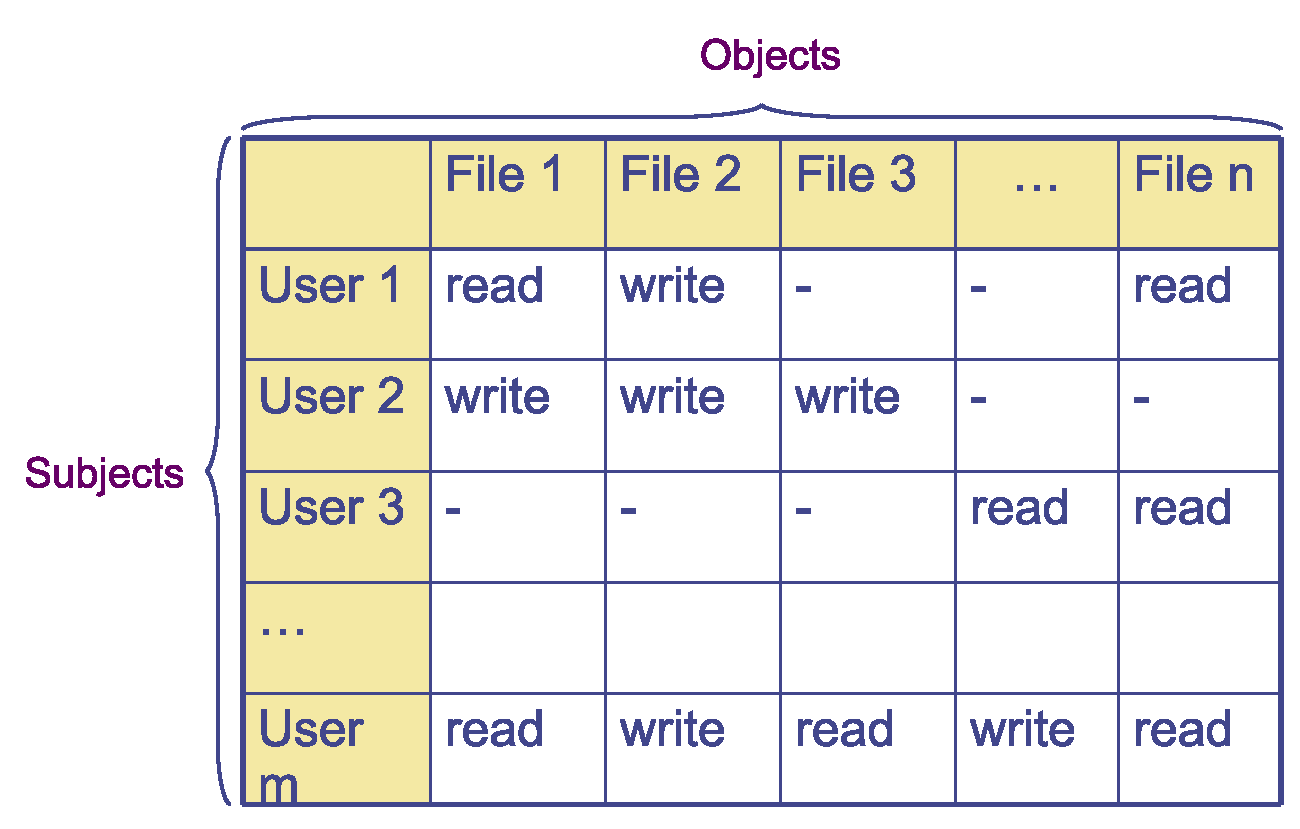
\includegraphics[width=4in]{figs/matrix}}
\end{slide}

\begin{slide}{Capabilities}
\vspace*{-.1in}
\itms{
  \item Slicing matrix along rows yields capabilities
  \ittms{
    \item E.g., For each process, store a list of objects it can access
    \item Process explicitly invokes particular capabilities
  }
  \item Can help avoid confused deputy problem
  \ittms{
    \item E.g., Must give compiler an argument that both specifies the
          output file and conveys the capability to write the file \\
	  (think about passing a file descriptor, not a file name)
    \item So compiler uses no \emph{ambient authority} to write file
  }
  \item Three general approaches to capabilities:
  \ittms{
    \item Hardware enforced (Tagged architectures like
      \cref{sched/readings/m-machine.pdf}{M-machine})
    \item Kernel-enforced
      (\cref{sched/readings/hydra.pdf}{Hydra},
      \href{http://www.cis.upenn.edu/~KeyKOS/NanoKernel/NanoKernel.html}{KeyKOS})
    \item Self-authenticating capabilities (like
      \href{http://www.cs.vu.nl/pub/amoeba/Intro.pdf}{Amoeba})
  }
  \item Good history in
    \href{http://www.cs.washington.edu/homes/levy/capabook/}{[Levy]}
}
\end{slide}

\begin{slide}{Hydra
\cref{sched/readings/hydra.pdf}{[Wulf]}}
\itms{
  \item Machine \& programing env.\ built at CMU in '70s
  \item OS enforced object modularity with capabilities
  \ittms{
    \item Could only call object methods with a capability
  }
  \item Agumentation let methods manipulate objects
  \ittms{
    \item A method executes with the capability list of the object,
	  not the caller
  }
  \item Template methods take capabilities from caller
  \ittms{
    \item So method can access objects specified by caller
  }
}
\end{slide}

\begin{slide}{KeyKOS
\href{http://www.cis.upenn.edu/~KeyKOS/NanoKernel/NanoKernel.html}{[Bomberger]}}
\itms{
  \item Capability system developed in the early 1980s
  \item Goal:  Extreme security, reliability, and availability
  \item Structured as a ``nanokernel''
  \ittms{
    \item Kernel proper only 20,000 likes of C, 100KB footprint
    \item Avoids many problems with traditional kernels
    \item Traditional OS interfaces implemented outside the kernel \\
          (including binary compatibility with existing OSes)
  }
  \item Basic idea:  No privileges other than capabilities
  \ittms{
    \item Means kernel provides purely \emph{objective} security mechanism
    \item As objective as pointers to objects in OO languages
    \item In fact, partition system into many processes akin to objects
  }
}
\end{slide}

\begin{slide}{Unique features of KeyKOS}
\itms{
  \item Single-level store
  \ittms{
    \item Everything is persistent:  memory, processes, \ldots
    \item System periodically checkpoints its entire state
    \item After power outage, everything comes back up as it was \\
          (may just lose the last few characters you typed)
  }
  \item ``Stateless'' kernel design only caches information
  \ittms{
    \item All kernel state reconstructible from persistent data
  }
  \item Simplifies kernel and makes it more robust
  \ittms{
    \item Kernel never runs out of space in memory allocation
    \item No message queues, etc.\ in kernel
    \item Run out of memory?  Just checkpoint system
  }
}
\end{slide}

\begin{slide}{KeyKOS capabilities}
\itms{
  \item Refered to as ``keys'' for short
  \item Types of keys:
  \ittms{
    \item \emph{devices} -- Low-level hardware access
    \item \emph{pages} -- Persistent page of memory (can be mapped)
    \item \emph{nodes} -- Container for 16 capabilities
    \item \emph{segments} -- Pages \& segments glued together with nodes
    \item \emph{meters} -- right to consume CPU time
    \item \emph{domains} -- a thread context
  }
  \item Anyone possessing a key can grant it to others
  \ittms{
    \item But creating a key is a privileged operation
    \item E.g., requires ``prime meter'' to divide it into submeters
  }
}
\end{slide}

\begin{slide}{Capability details}
\itms{
  \item Each domain has a number of key ``slots'':
  \ittms{
    \item 16 general-purpose key slots
    \item \emph{address slot} -- contains segment with process VM
    \item \emph{meter slot} -- contains key for CPU time
    \item \emph{keeper slot} -- contains key for exceptions
  }
  \item Segments also have an associated keeper
  \ittms{
    \item Process that gets invoked on invalid reference
  }
  \item Meter keeper (allows creative scheduling policies)
  \item Calls generate return key for calling domain
  \ittms{
    \item (Not required---other forms of message don't do this)
  }
}
\end{slide}

\begin{slide}{KeyNIX:  UNIX on KeyKOS} 
\itms{
  \item ``One kernel per process'' architecture
  \ittms{
    \item Hard to crash kernel
    \item Even harder to crash system
  }
  \item A process's kernel is its keeper
  \ittms{
    \item Unmodified Unix binary makes Unix syscall
    \item Invalid KeyKOS syscall, transfers control to Unix keeper
  }
  \item Of course, kernels need to share state
  \ittms{
    \item Use shared segment for process and file tables
  }
}
\end{slide}

\tikzset{
    myshade/.style={top color=white, bottom color=#1!10,
        shading angle=30, draw=#1!50,
        drop shadow={shadow xshift=.25ex,shadow yshift=-.25ex}},
    myshade/.default=black
}

\begin{frame}
\frametitle{KeyNIX overview}
\centerline{\scriptsize\openup-1\jot
\begin{tikzpicture}[node distance=1em,
    kdomain/.value forbidden,
    kdomain/.style={myshade,ellipse,align=center, text depth=0pt },
    driver/.style={kdomain}, inode/.style={kdomain}, unix/.style={kdomain},
    segment/.style={align=center,draw,inner sep=1.5ex},
    file/.style={segment,myshade},
    unix seg/.style={myshade,segment}
    ]
\node[driver] (dd1) {Device \\ Driver \\ Domain};
\node[driver,right=of dd1] (dd2) {Device \\ Driver \\ Domain};
\node[driver,right=of dd2] (dd3) {Device \\ Driver \\ Domain};
\node[driver,below=of dd2] (dd4) {Device \\ Table \\ Domain};
\path (dd4) edge (dd1) edge (dd2) edge (dd3);
\node[above=of dd1.west |- dd1.north,anchor=west] (dd0) {Device System};
\begin{scope}[on background layer]
\node[fit={(dd0) (dd1) (dd3) (dd4)}, inner sep=1em, on background layer,
    rounded corners,fill=blue!10!white] (devsystem) {};
\end{scope}
\node[inode,right=1cm of devsystem] (btree) {Btree\\ Domain};
\node[inode,right=of btree] (i2) {Inode\\ Domain};
\node[inode,above=of i2] (i1) {Inode\\ Domain};
\node[inode,below=of i2] (i3) {Inode\\ Domain};
\node[inode,anchor=70] at ([shift=(250:1em)] btree.250) (i4) {Inode\\ Domain};
\node[file,right=of i1] (f1) {File} edge (i1);
\node[file,right=of i2] (f2) {File} edge (i2);
\node[file,right=of i3] (f3) {File} edge (i3);
\path (btree) edge (i1) edge (i2) edge (i3) edge (i4);
\node[anchor=north west] (i0) at (i4.west |- i1.north) {File System};
\begin{scope}[on background layer]
\node[fit={(i0) (i4) (f1) (f3)}, inner sep=1em,
    on background layer,
    rounded corners,fill=cyan!10!white] (filesystem) {};
\end{scope}
\tikzset{node distance=1.5em}
\node[unix,anchor=west,below left=9mm and 8mm of filesystem.south west]
   (ukeeper) {UNIX\\ Keeper};
\node[unix] (qdom) at ([shift=(200:2cm)] ukeeper) {Queue\\Domain}
   edge (ukeeper);
\node[unix] (stdom) at ([shift=(-45:1.75cm)] qdom)
     {Sleep\\Timer\\Domain} edge (qdom) edge (ukeeper);
\node[unix] (proc) at ([shift=(-30:1.75cm)] ukeeper) {UNIX\\Process}
   edge (ukeeper);
\node[unix seg,right=of proc] (addrspace) {Address Space\\Segment}
   edge (proc);
\node[unix,anchor=south west] (segkeeper)
     at ([shift=(30:1em)] addrspace.north east)
     {Segment\\Keeper} edge (addrspace);
\begin{scope}[on background layer]
\node[fit={(ukeeper) (stdom) (segkeeper) (qdom)},on background layer,
    inner sep=1em,
    fill=violet!10!white,draw=violet!50,double copy shadow] (unix) {};
\end{scope}
\node[unix seg,left=.5em of unix.north west,anchor=north east] (ftab)
     {Process\\and\\Open File\\Table};
\path[draw=white,double=black,double distance=\pgflinewidth]
    (ukeeper) -- (dd4) (ukeeper) -- (i4)
    (ukeeper) -- (ftab);
\node[file,anchor=south west] (seg)
     at ([yshift=.25ex] unix.south -| dd1.west) {segment};
\node[inode,above=2ex of seg] (dom) {domain};
\end{tikzpicture}}
\end{frame}

%% \begin{slide}{KeyNIX overview} 
%% \vspace*{-.15in}
%% \centerline{\input{keynix}}
%% \end{slide}

\begin{slide}{Keynix I/O}
\itms{
  \item Every file is a different process
  \ittms{
    \item Elegant, and fault isolated
    \item Small files can live in a node, not a segment
    \item Makes the \texttt{namei()} function very expensive
  }
  \item Pipes require queues
  \ittms{
    \item This turned out to be complicated and inefficient
    \item Interaction with signals complicated
  }
  \item Other OS features perform very well, though
  \ittms{
    \item E.g., fork is six times faster than Mach 2.5
  }
}
\end{slide}

\begin{slide}{Self-authenticating capabilities}
\itms{
  \item Every access must be accompanied by a capability
  \ittms{
    \item For each object, OS stores random \emph{check} value
    \item Capability is:
          $\{\hbox{Object},\hbox{Rights},\textsc{mac}
      (\mathit{check},\hbox{Rights})\}$ \\
    (\textsc{mac} = cryptographic \emph{Message Authentication
        Code})
  }
  \item OS gives processes capabilities
  \ittms{
    \item Process creating resource gets full access rights
    \item Can ask OS to generate capability with restricted rights
  }
  \item Makes sharing very easy in distributed systems
  \item To revoke rights, must change \emph{check} value
  \ittms{
    \item Need some way for everyone else to reacquire capabilities
  }
  \item Hard to control propagation
}
\end{slide}

\begin{slide}{Amoeba}
\itms{
  \item A distributed OS, based on capabilities of form:
  \ittms{
    \item server port, object ID, rights, check
  }
  \item Any server can listen on any machine
  \ittms{
    \item Server port is hash of secret
    \item Kernel won't let you listen if you don't know secret
  }
  \item Many types of object have capabilities
  \ittms{
    \item Files, directories, processes, devices, servers (E.g., X windows)
  }
  \item Separate file and directory servers
  \ittms{
    \item Can implement your own file server, or store other object
      types in directories, which is cool
  }
  \item Check is like a secret password for the object
  \ittms{
    \item Server records check value for capabilities with all rights
    \item Restricted capability's check is hash of old check, rights
  }
}
\end{slide}

\begin{slide}{Limitations of capabilities}
\itms{
%  \item IPC performance, as we've discussed
  \item IPC performance a losing battle with CPU makers
  \ittms{
    \item CPUs optimized for ``common'' code, not context switches
    \item Capability systems usually involve many IPCs
  }
  \item Capability model never took off as kernel API
  \ittms{
    \item Requires changes throughout application software

    \item Call capabilities ``file descriptors'' or ``Java pointers''
	  and people will use them

    \item But discipline of pure capability system challenging so far

    \item People sometimes quip that capabilities are an OS concept of
	  the future and always will be
  }
  \item Language-level object capabilities in use by Firefox
}
\end{slide}


\end{document}

\begin{slide}{DAC vs.\ MAC}
\itms{
  \item Most people familiar with discretionary access control (DAC)
  \ittms{
    \item Unix permission bits are an example
    \item Might set a file \texttt{private} so only group
      \texttt{friends} can read it
  }
  \item Discretionary means anyone with access can propagate
  information:
  \ittms{
    \item \texttt{Mail sigint@enemy.gov < private}
  }
  \item Mandatory access control
  \ittms{
    \item Security administrator can restrict propagation
    \item Abbreviated MAC (NOT a message authentication code)
  }
}
\end{slide}

\begin{slide}{Bell-Lapadula model}
%[9in,7.5in]
\itms{
  \item View the system as subjects accessing objects
  \ittms{
    \item The system input is requests, the output is decisions
    \item Objects can be organized in one or more hierarchies, $H$\\
	  (a tree enforcing the type of decendents)
  }
  \item Four modes of access are possible:
  \ittms{
     \item \Red{\underline{\Black{e}}}xecute -- no observation or alteration
     \item \Red{\underline{\Black{r}}}ead -- observation
     \item \Red{\underline{\Black{a}}}ppend -- alteration
     \item \Red{\underline{\Black{w}}}rite -- both observation and modification
  }
  \item The current access set, $b$, is (subj, obj, attr) tripples
  \item An access matrix $M$ encodes permissible access types
        (as before, subjects are rows, objects columns)
%  \ittms{
%    \item C.f., reference/access graph from capability systems
%  }
}
\end{slide}

\begin{slide}{Security levels}
\itms{
  \item A \emph{security level} is a $(c,s)$ pair:
  \ittms{
    \item $c=$ classification -- E.g., unclassified, secret, top secret
    \item $s=$ category-set -- E.g., Nuclear, Crypto
  }
  \item $(c_1,s_1)$ \emph{dominates} $(c_2,s_2)$ iff $c_1\ge c_2$
    and $s_2\subseteq s_1$
  \ittms{
    \item $L_1$ \emph{dominates} $L_2$ sometimes written $L_1\sqsupseteq L_2$
           or $L_2\sqsubseteq L_1$
    \item levels then form a lattice
  }
  \item Subjects and objects are assigned security levels
  \ittms{
    \item level(S), level(O) -- security level of subject/object
    \item current-level(S) -- subject may operate at lower level
    \item level(S) bounds current-level(S) (current-level(S)
    $\sqsubseteq$ level(S))
    \item Since level(S) is max, sometimes called S's \emph{clearance}
%    \item $f=(\mathrm{level}, \mathrm{level}, \mathrm{current\hyph level})$
  }
%  \item State of system is 4-tuple $(b,M,f,H)$
}
\end{slide}

\begin{slide}{Security properties}
\itms{
  \item The simple security or \emph{ss-property}:
  \ittms{
    \item For any $(S,O,A)\in b$, if $A$ includes observation, then
	  level($S$) must dominate level($O$)
    \item E.g., an unclassified user cannot read a top-secret document
  }
  \item The star security or \emph{*-property}:
  \ittms{
    \item If a subject can observe $O_1$ and modify $O_2$, then
	  level($O_2$) dominates level($O_1$)
    \item E.g., cannot copy top secret file into secret file
    \item More precisely, given $(S,O,A)\in b$: \\
      if $A=r$ then current-level($S$) $\sqsupseteq$ level($O$) (``no
      read up'') \\
      if $A=a$ then current-level($S$) $\sqsubseteq$ level($O$) (``no
      write down'')\\
      if $A=w$ then current-level($S$) $=$ level ($O$)
%          level($O$) dominates current-level($S$) if $A=a$\\
%          level($O$) is current-level($S$) if $A=w$\\
%          level($O$) is dominated by current-level($S$) if $A=r$
  }
}
\end{slide}

\begin{slide}{Straw man MAC implementation}
\itms{
  \item Take an ordinary Unix system
  \item Put labels on all files and directories to track levels
  \item Each user U has a security clearance (level(U))
  \item Determine current security level dynamically
  \ittms{
    \item When U logs in, start with lowest curent-level
    \item Increase current-level as higher-level files are observed \\
             (sometimes called a \emph{floating label} system)
    \item If U's level does not dominate current, kill program
    \item If program writes to file it doesn't dominate, kill it
  }
  \item Is this secure?
}
\end{slide}

\begin{slide}{No:  Covert channels}
\itms{
  \item System rife with \emph{storage channels}
  \ittms{
    \item Low current-level process executes another program
    \item New program reads sensitive file, gets high current-level
    \item High program exploits covert channels to pass data to low
  }
  \item E.g., High program inherits file descriptor
  \ittms{
    \item Can pass 4-bytes of information to low prog.\ in file offset
  }
%  \item Labels themselves can be a storage channel
%  \ittms{
%    \item Arrange to raise process $p_i$'s label to communicate $i$
%  }
  \item Other storage channels:
  \ittms{
    \item Exit value, signals, file locks, terminal escape codes, \ldots
  }
  \item If we eliminate storage channels, is system secure?
}
\end{slide}

\begin{slide}{No:  Timing channels}
\itms{
  \item Example:  CPU utilization
  \ittms{
    \item To send a 0 bit, use 100\% of CPU is busy-loop
    \item To send a 1 bit, sleep and relinquish CPU
    \item Repeat to transfer more bits
  }
  \item Example:  Resource exhaustion
  \ittms{
   \item High prog.\ allocate all physical memory if bit is 1
   \item If low prog.\ slow from paging, knows less memory available
  }
  \item More examples:  Disk head position, processor cache/TLB
    polution, \ldots
}
\end{slide}

\begin{slide}{Reducing covert channels}
\itms{
  \item Observation:  Covert channels come from sharing
  \ittms{
    \item If you have no shared resources, no covert channels
    \item Extreme example:  Just use two computers
  }
  \item Problem:  Sharing needed
  \ittms{
    \item E.g., read unclassified data when preparing classified
  }
  \item Approach:  Strict partitioning of resources
  \ittms{
    \item Strictly partition and schedule resources between levels
    \item Occasionally reapportion resources based on usage
    \item Do so infrequently to bound leaked information
    \item In general, only hope to bound bandwidth of covert channels
    \item Approach still not so good if many security levels possible
  }
}
\end{slide}

\begin{slide}{Declassification}
\itms{
  \item Sometimes need to prepare unclassified report from classified
    data
  \item Declassification happens outside of system
  \ittms{
    \item Present file to security officer for downgrade
  }
  \item Job of declassification often not trivial
  \ittms{
    \item E.g., Microsoft word saves a lot of undo information
    \item This might be all the secret stuff you cut from document
  }
}
\end{slide}



\end{document}
